\documentclass[main.tex]{subfiles}

\begin{document}

	\begingroup

	\renewcommand{\cleardoublepage}{}

	\renewcommand{\clearpage}{}

	\chapter{Clean Up Task Overview}

		\chapterauthor{Torge Olliges, Jan Schimpf}
		
		\section{Goal}
		For Clean Up the HSR had to navigate a room in which objects are distributed. The robot has no prior knowledge of the position of the objects but it does know the position of the goal which was a bucket. It had to be able to detect the objects in the room pick them up and transport them to the designated goal position. The HSR had to achieve the tasks given autonomously and manipulate objects like the objects explained in the goal section of the Clean Up task chapter. It had 5 minutes to achieve this task.
		

	  	\section{Tasks}
	  	\subsection{Setup}
	First the interface to knowledge is called to set the target to basket. In addition, the floor and the table are set as sources, since objects are picked up from both. Since knowledge is responsible for the internal representation of the surfaces and the management of the associated objects, we have to tell them from where we will pick up objects and where they will be taken. 
	  	\begin{figure}	
	  		\centering
	  		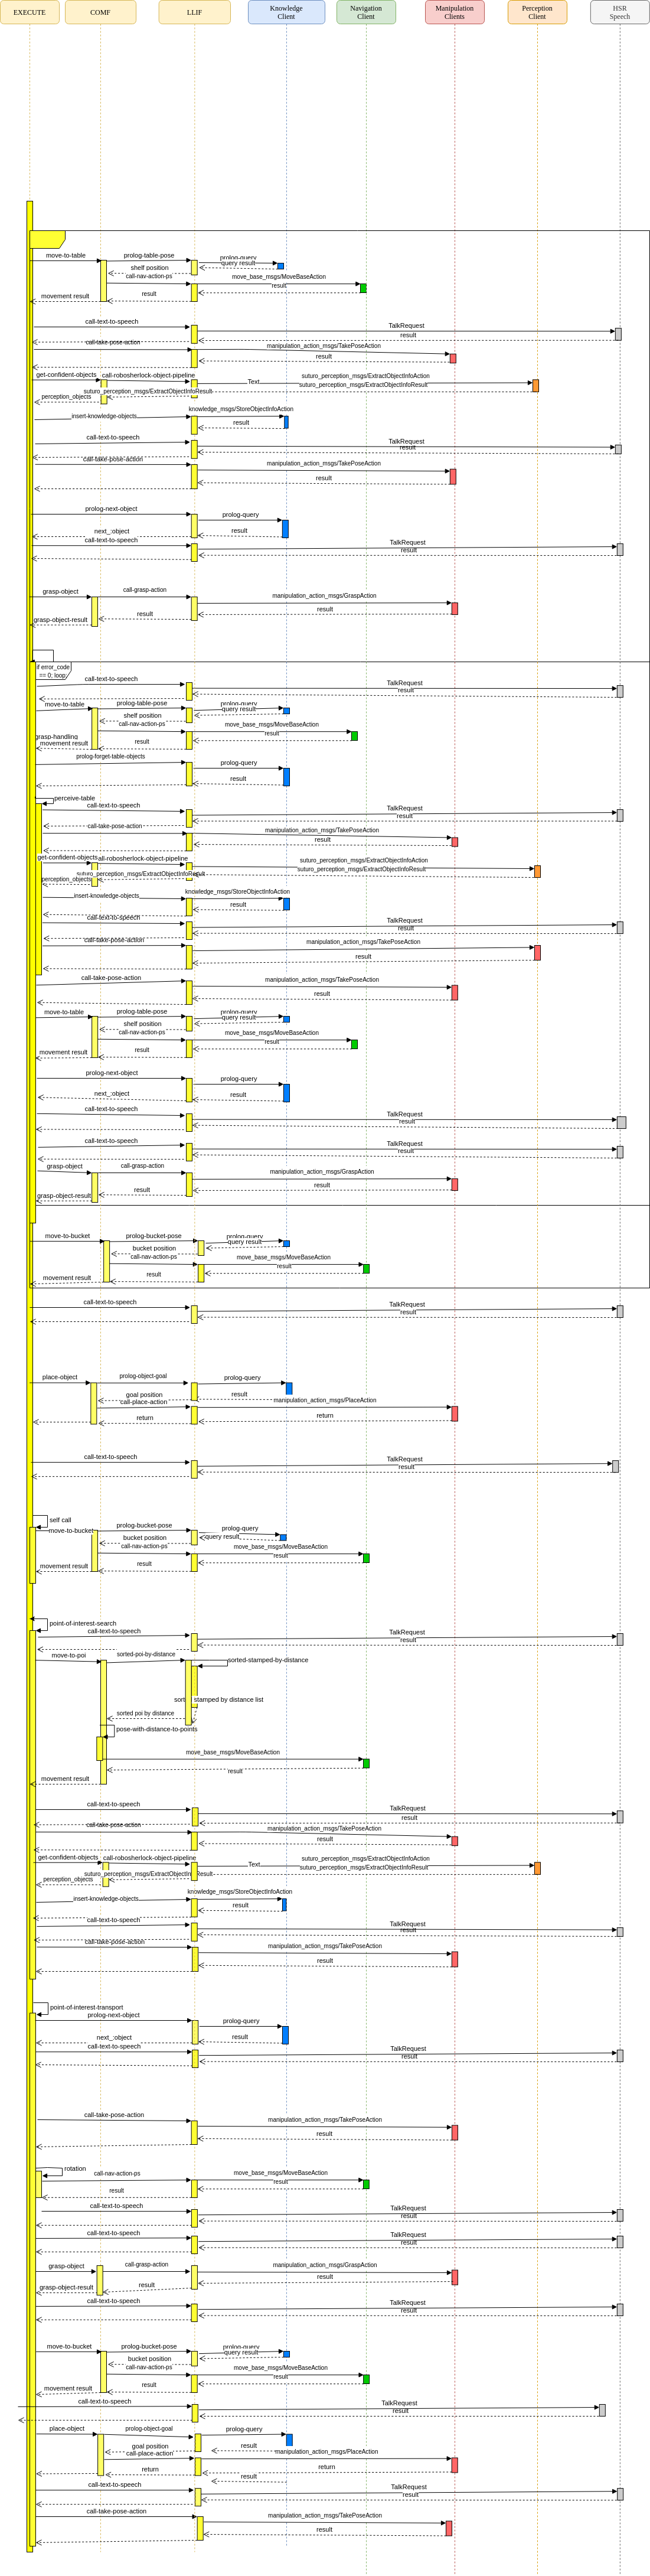
\includegraphics[width=0.85\textwidth]{pictures/diagramms/cleanup-sequence.png}
	  		\caption{Sequence diagram of the complete run of the clean up task \textit{(explanations below)}}
	  		\label{Clean Up sequence}
	  	\end{figure}
		% TODO: Entfernen - hier bitte aus dem sequenz diagramm einen einzelnen task als subsection z.b. schritt: tür öffnen, dafür mussten perception dies tun manipulation das tun etc.
		

	\subsection{Scan table sequence}
	% Manipulation: take pose action
	The robot is set to the default pose so it doesn't collide with any objects, this could happen if the robot is told to move while in a pose where for example the arm is extended.
	
	% NLP: Talk Request
	
	The talk requests are used to inform the developer as well as the people following the robot or evaluating its behavior about what the robot is about to do. They are also used for safety measures so the robot can warn when it is going to move so bystanders can step aside. 
	
	% Knowledge: get table-poses
	Knowledge finds all the tables available, sorts them by their distance to the robot and then returns the list of their position to Planning, so Planning can determine where to go next.
	
	% Navigation: moveBaseAction
	
	The robot moves to the designated location in this case the table, it will be turned $90^\circ$ so it is in a pose where perceiving the table isn't hindered by the arm of the HSR. 
	
	% NLP
	Informing that the robot is perceiving the table now.
	
	% Manipuilation: TakePoseAction
	The robot has to take one of 3 perceive poses depending on the heights of the objects he wants to look at.
	
	% Perception: Percieve and return data
	The HSR takes a picture of the scene it is currently looking at and processes it with RoboSherlock. Based on the requested region the input images are filtered. The results are then published by the \textit{perception\_actionserver}.

	
	% Knowledge: Store Data
	Knowledge checks the data of the object, that is supposed to be stored. If the class is unknown to knowledge, it is set to other. If the data is valid the object gets added to the knowledge base and the objects at the position of the new object are put into a group.
	% NLP: Talk Request
	
	% Manipulation: Take pose
	Take default pose.
	
	% 2x NLP: Talk
		
	% Navigation: MoveBaseAction
	Turn the HSR by $90^\circ$ so he can grasp objects which would not be possible from the pose he took to perceive the objects.
	
	\subsection{Grasp sequence}
	
	%prolog-next-object
    The Knowledge base is queried for next Object that should be grasped.
	What the next object should be is determined by \textbf{KNOWLEDGE LEUTE MÜSSEN DAS ERKLÄREN}.	
	
	%NLP Grasping object
	Informing that the robot will now grasp an object
	%NLP Which object
	Informing which object the robot will grasp using the object id
	
	%grasp-object
	The object id is used to query the Knowledge base for the dimensions of the object and the pose of the object. The results are then used to call the manipulation grasp server to grasp the object. Manipulation then \textbf{MANIPULATION LEUTE MÜSSEN DAS ERKLÄREN}
	 %Knowledge: prolog dimensions
	 %Knowledge: prolog pose
	 
	%NLP succesfully grasped
	Informing that the robot has successfully grasped an object
    
	\subsection{Place sequence}
	%Navigation: moveBaseAction
	The robot moves to the designated location in this case the bucket.
	The coordinates for the navigation call are queried from the Knowledge base and adjusted so the robot looks at the bucket and can place the object inside it. 
	
	%NLP placing the object
	Informing that the robot is now placing the object

	%place-object
	The object id is used to querie the Knowledge base for the dimensions of the object and the goal of the object. The results are then used to call the manipulation place server to place the object. Manipulation then \textbf{MANIPULATION LEUTE MÜSSEN DAS ERKLÄREN}
	 %Knowledge: prolog dimensions
	 %Knowledge: prolog goal
	 
	%NLP placed the object
	Informing that the robot has successfully placed the object

	%Manipulation: Take pose
	Returns the robot into the default pose.
	
	This is looped for two times.
	The first one is for the table and stops if there are no more objects on it to be placed in the bucked. The sedon one is for the point of interest search and stops if there are not points of interest left.
	
	\subsection{Point of interest search sequence}
    %NLP found an point of interest to search
    Informing that the robot has found a point of interest to search for objects
    
    %move-to-poi
    The first set of coordinates from a list containing the coordinates of locations with that may have objects is used to move the robot into position to perceive it. 
    The list is created by looking at the returns of the laser scanner and overlapped with the obstacle map to filter out furniture and walls. 
    The Robot then takes a perceive position so it can perceive the floor.
    
    %NLP perceiving the postition
    Informing that the robot is now perceiving the position
      
    %call-robosherlock-object-pipeline
	The HSR takes a picture of the scene it is currently looking at and processes it with RoboSherlock. Based on the requested region the input images are filtered. The results are then published by the \textit{perception\_actionserver}.

    
    %Knowledge:insert-knowledge-objects
    Knowledge checks the data of the object, that is supposed to be stored. If the class is unknown to knowledge, it is set to other. If the data is valid the object gets added to the knowledge base and the objects at the position of the new object are put into a group.
    
    %call-take-pose-action
   	Returns the robot into the default pose to be able to grasp the object.

    % Navigation: MoveBaseAction
    Turn the HSR by $90^\circ$ so he can grasp objects which would not be possible from     the pose he took to perceive the objects.

    After the place sequence that comes after this is identical to the one shown in \emph{5.2.3}
	\section{Conclusion}
		
		
	\endgroup

\end{document}
